\documentclass[10pt,xcolor=pdflatex,hyperref={unicode}]{beamer}
\usepackage{newcent}
\usepackage[utf8]{inputenc}
\usepackage[czech]{babel}
%\usepackage[T1]{fontenc}
\usepackage{hyperref}
\usepackage{fancyvrb}
\usetheme{FIT}
\usepackage{listings}

\lstdefinelanguage{Gherkin}{
	morekeywords = {
		Given,
		When,
		Then,
		And,
		Scenario,
		Feature,
		But,
		Background,
		Scenario Outline,
		Examples
	},
	sensitive=true,
	morecomment=[l]{\#},
	morestring=[b]",
	morestring=[b]'
}

%%%%%%%%%%%%%%%%%%%%%%%%%%%%%%%%%%%%%%%%%%%%%%%%%%%%%%%%%%%%%%%%%%
\title[Martin Krajňák - SEP]{Automatické generování testů pro GNOME GUI aplikace z metadat AT-SPI}

\author[]{Martin Krajňák}

\institute[]{Brno University of Technology, Faculty of Information Technology\\
Bo\v{z}et\v{e}chova 1/2. 612 66 Brno - Kr\'alovo Pole\\
xkrajn02@fit.vutbr.cz}

%\institute[]{Fakulta informačních technologií
%Vysokého učení technického v Brně\\
%Bo\v{z}et\v{e}chova 1/2. 612 66 Brno - Kr\'alovo Pole\\
%login@fit.vutbr.cz}

% České logo - Czech logo
% beamerouterthemeFIT.sty řádek 9: fitlogo1_cz

\date{January 26, 2020}
%\date{\today}
%\date{} % bez data / without date

%%%%%%%%%%%%%%%%%%%%%%%%%%%%%%%%%%%%%%%%%%%%%%%%%%%%%%%%%%%%%%%%%%

\begin{document}

\frame[plain]{\titlepage}

\begin{frame}\frametitle{Cieľ práce}
   
    
    \begin{block}{Nástroj na automatické generovanie automatizovaných testov}

    \begin{itemize}
    \item Systematické vytvorenie testov na základe dostupných vykonateľných akcií GUI aplikácie
        \begin{itemize}
        \item Testovanie častí nepokrytých manuálnym testovaním
        \item Vytvorenie testov vhodných na regresné testovanie počas vývoja aplikácie (aktualizácia backendu)
    \end{itemize}

    \item Využitie vstavenej podpory asistenčných technológii pre GTK/GNOME aplikácie
    \item Využitie technológie OCR
        \begin{itemize}
            \item Open Source technológia vyvíjaná Google
            \item rozpoznávanie znakov/textu z obrázkov
            \item verifikácia skutočného obsahu zobrazeného v aplikácii
        \end{itemize}
    \item zjednodušenie/zrýchlenie procesu vývoja a údržby automatizovaných testov
    \item rýchle zistenie závažných chýb 
    \end{itemize}

    \end{block}
\end{frame}

\begin{frame}\frametitle{Technológia AT-SPI a jej rozhrania}
    \begin{itemize}
        \item hlboko vstavaná do frameworku GTK, prítomná vo všetkých aplikáciach využívajúce grafické prvky GTK prípadne ich varianty
        \item ponúka strom prvkov aplikácie a ich:
        \begin{itemize}
            \item pozíciu
            \item viditeľnosť
            \item vykonateľné udalosti/akcie
            \item viditeľný text
        \end{itemize}
        \item dostupnosť prvkov v jazyku Python3 cez knižnice:
        \begin{itemize}
            \item pyatspi
            \item dogtail
        \end{itemize}
    \end{itemize}
\end{frame}

\begin{frame}\frametitle{Technológia AT-SPI - aplikácia Nautilus}
    \begin{figure}[h]
        \center{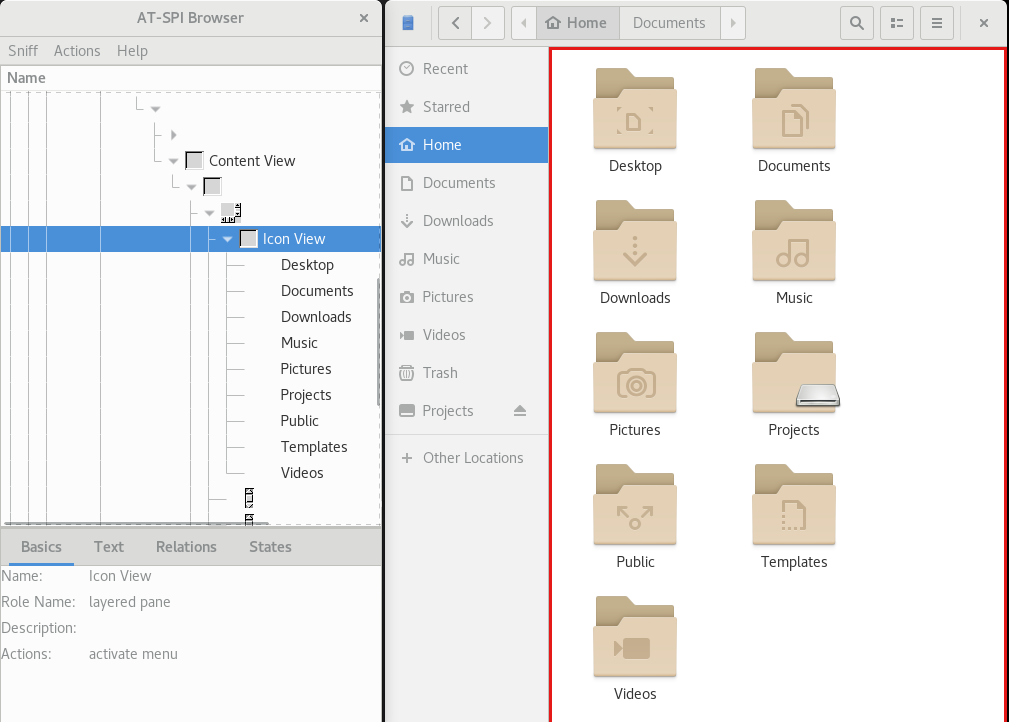
\includegraphics[scale=0.3]{img/sniff.png}}
        \label{sniff}
    \end{figure}
\end{frame}


\begin{frame}\frametitle{Extrakcia Modelu, Generovanie testov}
\begin{enumerate}
    \item Vytvorenie abstraktného modelu aplikácie na základe dát dostupných z AT-SPI
        \begin{enumerate}
        \item spustenie aplikácie
        \item zmapovanie udalostí dostupných v súčasnom stave
        \item postupné vytvorenie grafu udalostí (Control Flow/Event Flow graph)
    \end{enumerate}
    \item Výber a vykonanie udalosti
    \item Overovanie stavu aplikácie
    \begin{itemize}
        \item sledovanie chýb
        \item kontrola behu, detekcia nových okien, dialógov
        \item kontrola zobrazenia určitých prvkov cez AT-SPI, OCR (z ang. assertion) 
    \end{itemize}
    \item Vygenerovanie kroku testu (behave step)
\end{enumerate}

    \begin{figure}[h]
        \center{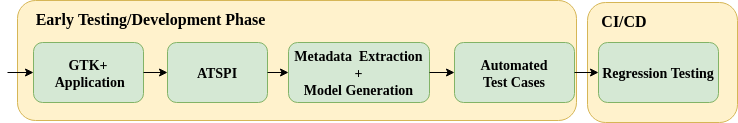
\includegraphics[scale=0.42]{img/diagram.png}}
        \label{diagram}
    \end{figure}
\end{frame}


\begin{frame}\frametitle{Výzvy}
    \begin{enumerate}
        \item určenie optimálneho konca testu (dĺžka sekvencie udalostí)
        \item vyhodnotenie pokrytia udalostí testami
        \item detekcia a začlenenie novo vzniknutých časti stromu počas generovania
        \item detekcia zmien v strome medzi jednotlivými udalosťami
        \item filtrovanie dialógov(výber súboru zo súborového systému, výber tlačiarne, otvorenie webovej stránky)
        \begin{itemize}
            \item vytvorenie kópie celého/časti stromu len s konkrétnymi vlastnosťami 
        \end{itemize}
        \item reakcie na chyby počas generovania/označenie chyby aby sa jej generátor vyhol
        \item začlenenie klávesových skratiek do testov
        \item začlenenie ostatných udalostí(pravý klik, položky kontextového menu)
    \end{enumerate}
\end{frame}

\begin{frame}[fragile]\frametitle{Ukážka testu}

\begin{lstlisting}[language=Gherkin]

Feature: Start and stop baobab in different ways

  @startViaCommand
  Scenario: Start via command
    Given Start baobab via command in session
    Then baobab should start
\end{lstlisting}
\begin{figure}[h]
    \center{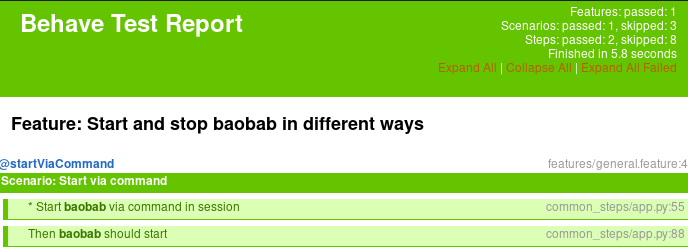
\includegraphics[scale=0.42]{img/behave_report.png}}
    \label{diagram}
\end{figure}

\end{frame}


\bluepage{
Ďakujem za pozornosť
}

\end{document}
